\documentclass{article}
\usepackage{ctex}
\usepackage{tikz}

\usetikzlibrary{decorations.pathreplacing}


\begin{document}
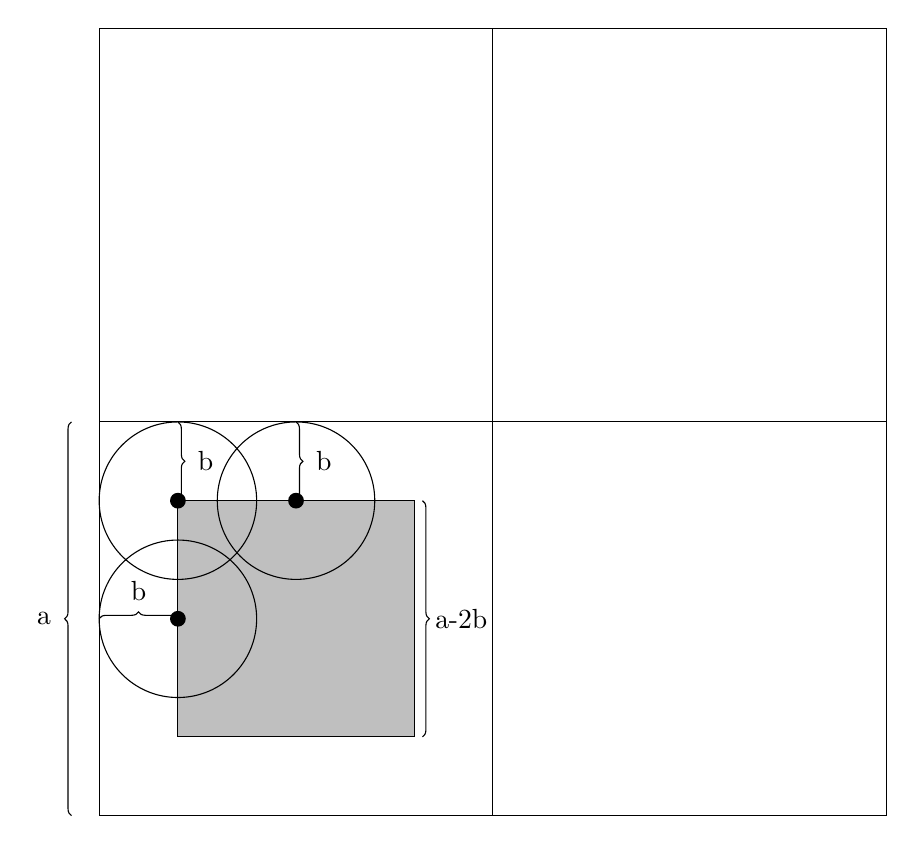
\begin{tikzpicture}
    
    \coordinate (A1) at (0,5);
    \coordinate (A2) at (5,0);
    \coordinate (B1) at (0+1, 5-1);
    \coordinate (B2) at (5-1, 0+1);
    \coordinate (C1) at (5/2, 5-1);
    \coordinate (C2) at (0+1, 5/2);
    
\draw (A1) rectangle (A2);
\draw[fill=lightgray] (B1) rectangle (B2);
\draw (B1) circle (1);
\draw (C1) circle (1);
\draw (C2) circle (1);
\draw (0,10) rectangle (5,5);
\draw (5,10) rectangle (10,5);
\draw (5,5) rectangle (10,0);

\fill (B1) circle (.1);
\fill (C1) circle (.1);
\fill (C2) circle (.1);

\draw[decorate, decoration={brace,mirror,raise=10pt}] (A1)--(0,0) node[midway, xshift=-20pt]{a};
\draw[decorate, decoration={brace,mirror,raise=0pt}] (B1)--(1,5) node[midway, xshift=10pt]{b};
\draw[decorate, decoration={brace,mirror,raise=0pt}] (C1)--(2.5,5) node[midway, xshift=10pt]{b};
\draw[decorate, decoration={brace,mirror,raise=0pt}] (C2)--(0,2.5) node[midway, yshift=10pt]{b};
\draw[decorate, decoration={brace,mirror,raise=3pt}] (4,1)--(4,4) node[midway, xshift=17pt]{a-2b};



\end{tikzpicture}
\end{document}